% Slides for 2025-07-01
% To create a slide, use the following:
% \begin{frame}{TITLE}
%     BODY
% \end{frame}

% To create a slide with a bullet list, use the following:
% \begin{frame}{TITLE}
%     \begin{itemize}
%         \item ITEM 1
%         \item ITEM 2
%     \end{itemize}    
% \end{frame}

% To create a slide with numbered list, use the following:
% \begin{frame}{TITLE}
%     \begin{enumerate}
%         \item ITEM 1
%         \item ITEM 2
%     \end{enumerate}
% \end{frame}

% To create a slide with a graphic:
% 1. Add the graphic to this folder (named picture.png)
% 2. Use the following:
% \begin{frame}{TITLE}
%     \centering
%     \includegraphics[height=0.7\textheight,width=0.7\textwidth,keepaspectratio]{picture.png}
% \end{frame}

% To create a slide with two columns, use the following:
% \begin{frame}{TITLE}
%     \begin{columns}
%         \begin{column}{0.5\textwidth}
%             COLUMN 1 BODY
%         \end{column}
%         \begin{column}{0.5\textwidth}
%             COLUMN 2 BODY
%         \end{column}
%     \end{columns}
% \end{frame}

\begin{frame}{MM ML - What We Have So Far}
    \begin{itemize}
        \item ResNet-UNet model performs binary segmentation on 3-channeled RGB high resolution drone imagery
    \end{itemize}
    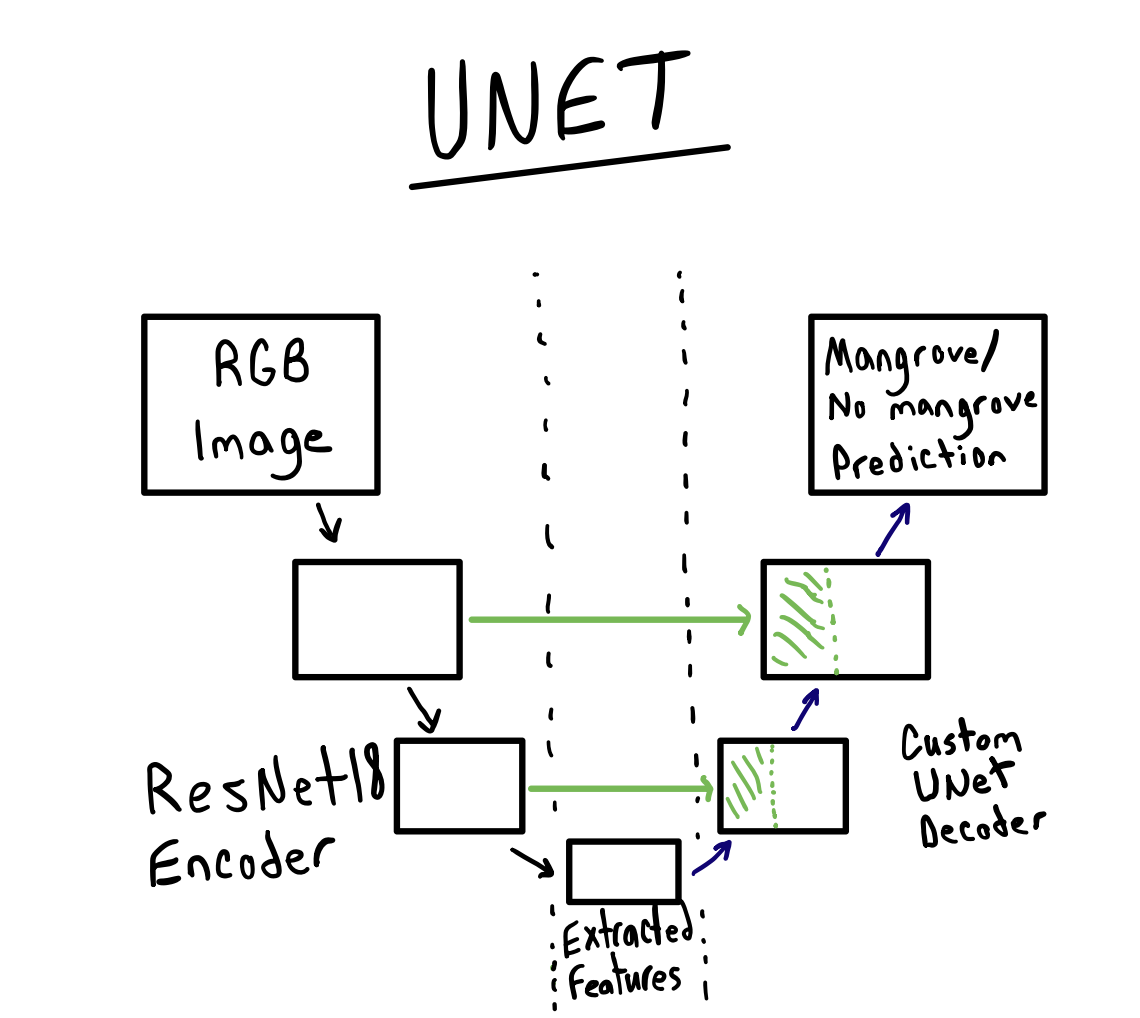
\includegraphics[height=0.7\textheight,width=0.7\textwidth,keepaspectratio]{images/unet.png}
\end{frame}

\begin{frame}{High Level Goals For Summer}
  \begin{itemize}
      \item Create diffusion dataset consisting of drone image TO label TO satellite image tile triplets
      \item Expand diffusion dataset with publically available high-resolution geospatial imagery
      \item Train diffusion model on latent space
      \item Train ResNet-UNet-Diffusion model, benchmark results
  \end{itemize}
\end{frame}

\begin{frame}{ResNet-UNet-Diffusion}
    \centering
    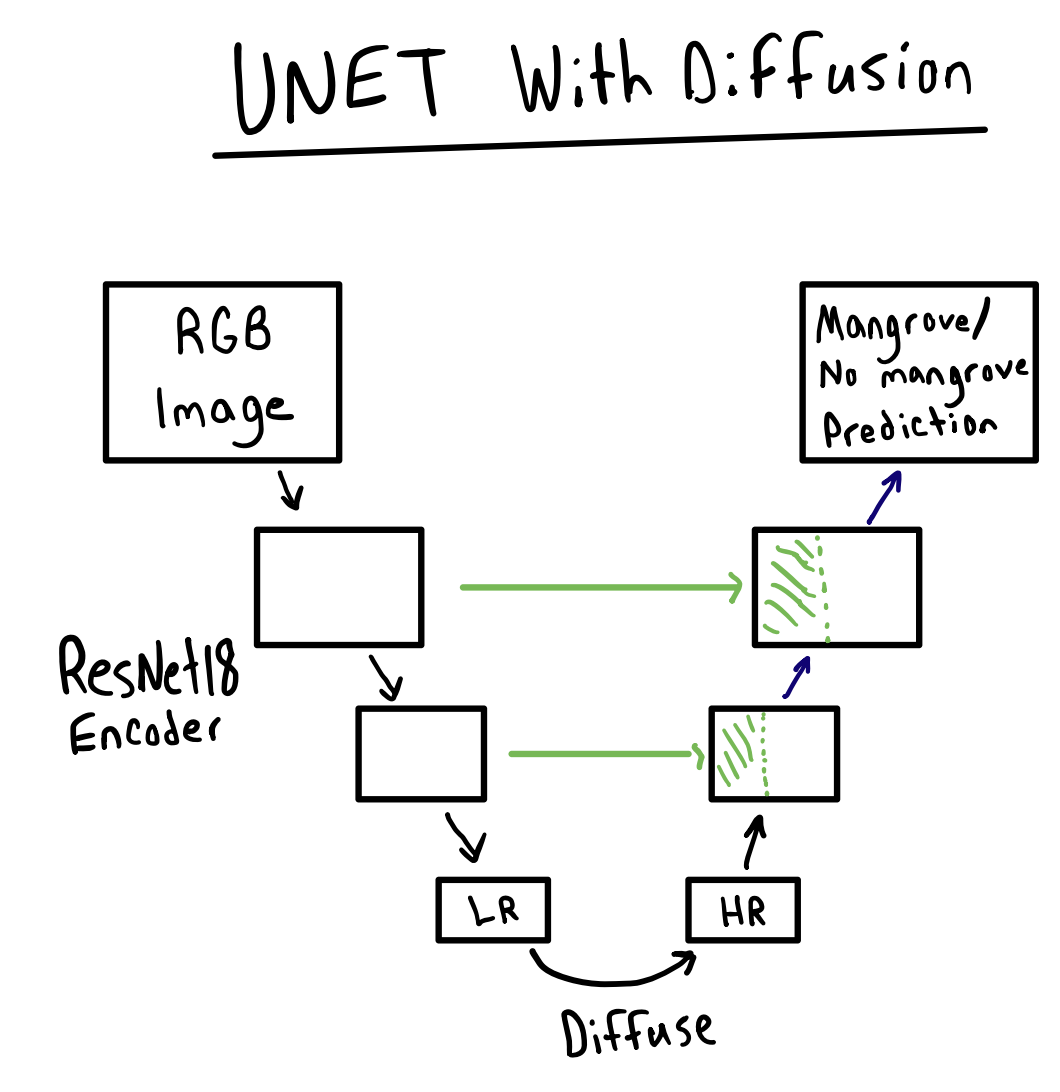
\includegraphics[height=0.7\textheight,width=0.7\textwidth,keepaspectratio]{images/unet-diffusion.png}
\end{frame}

\begin{frame}{Drone VS Satellite}
  \centering
  \begin{minipage}{0.48\textwidth}
    \centering
    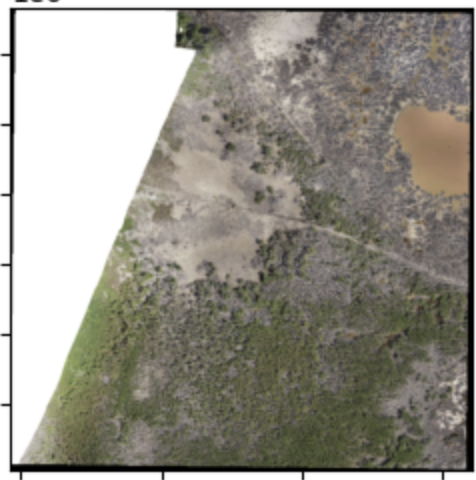
\includegraphics[width=\textwidth,keepaspectratio]{images/chunk-tif.png}
    \textbf{Drone}
  \end{minipage}
  \hfill
  \begin{minipage}{0.48\textwidth}
    \centering
    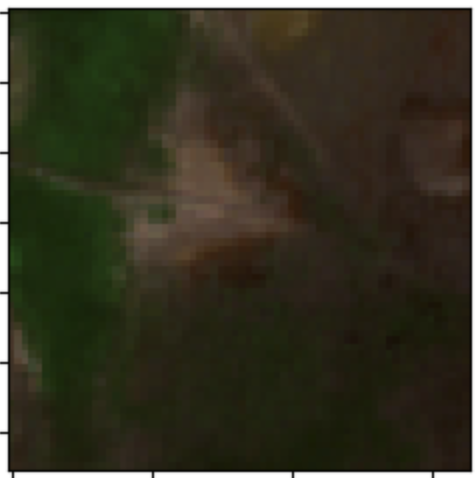
\includegraphics[width=\textwidth,keepaspectratio]{images/satellite-tif.png}
    \textbf{Satellite}
  \end{minipage}
\end{frame}

\begin{frame}{Satellite Bands}
  \centering
  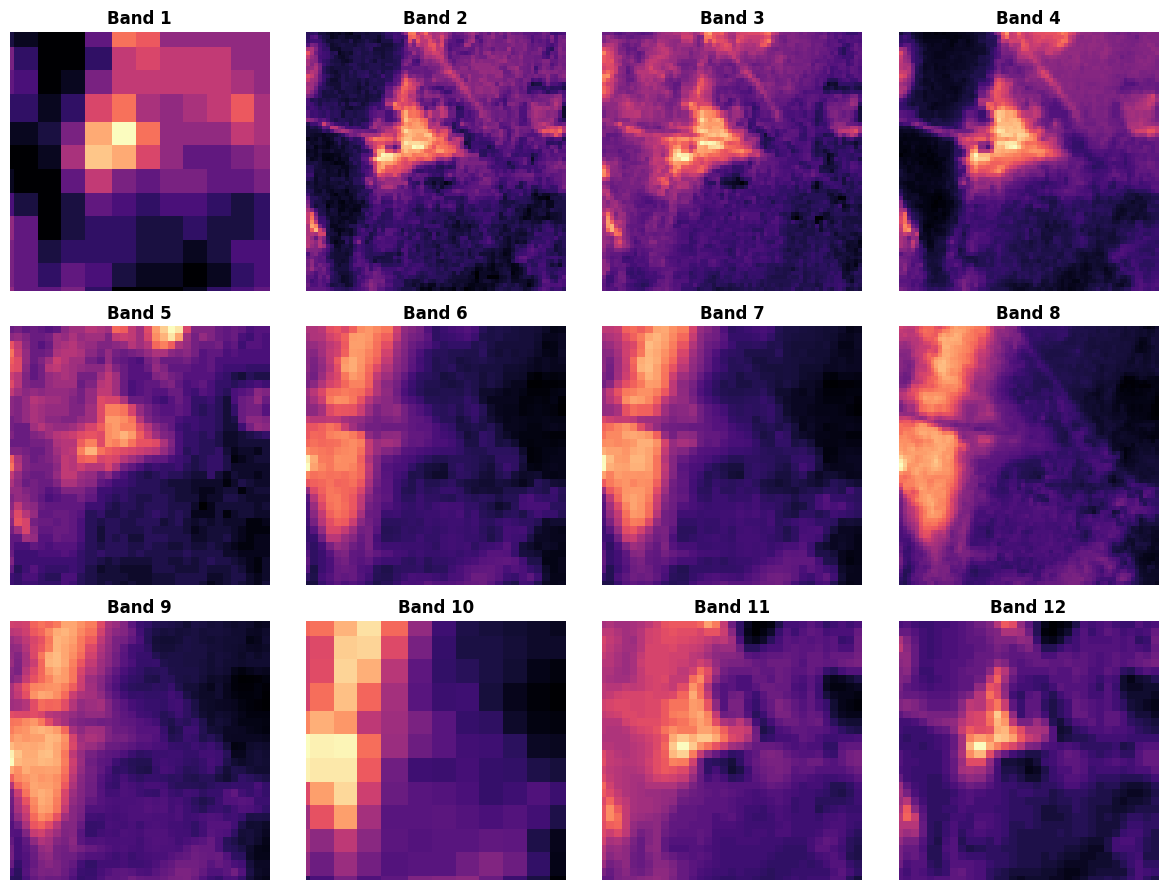
\includegraphics[height=0.7\textheight,width=0.7\textwidth,keepaspectratio]{images/satellite-bands.png}
\end{frame}

\begin{frame}{Next Week}
  \begin{itemize}
      \item Dataset creation workflow. Get satellite imagery through Sentinel Hub API
      \item Search online for additional high-resolution geospatial data
      \item Rescale and tile image files
      \item Get data on NAS
  \end{itemize}
\end{frame}

